%!TEX root = widefieldscan.tex
\svnidlong
{$HeadURL$}
{$LastChangedDate$}
{$LastChangedRevision$}
{$LastChangedBy$}
%
%\ifhtml
%\else
%\begin{center}
%	\fbox{
%		\begin{minipage}{.618\columnwidth}
%		The section below is versioned at \url{\svnkw{HeadURL}} (last commit @ \svnfileday.\svnfilemonth.\svnfileyear \space \svnfilehour:\svnfileminute, Revision: \svnkw{LastChangedRevision}).
%		\end{minipage}
%	} 
%\end{center}
%\fi
%
\section{Results}\label{sec:Results}%
\subsection{Image Merging and Reconstruction}\label{sec:Image Merging and Reconstruction}%
Multiple independently acquired projection images covering the desired field of view have been merged into single projections covering the full field of view. Figure~\ref{fig:wide field scan results}(a) shows corrected projection images from three overlapping subscans prior to merging (with marked overlapping regions). Figure~\ref{fig:wide field scan results}(b) shows one merged projection image prior to reconstruction and figure~\ref{fig:wide field scan results}(c) shows one slice of the reconstructed dataset of protocol B, acquired from 5244 projections. Such a reconstructed slice covers a field of view of 2792$\times$2792 pixels (4.13$\times$\SI{4.13}{\milli\meter}) which is almost three times the size of what can be achieved with one single binned scan (1024 pixels or \SI{1.52}{\milli\meter}). %1024 * 1.48 um/px = 1.51552mm

\ifiucr
	\begin{figure}%
			\caption{Wide field scan of a rat lung sample obtained from a Sprague-Dawley rat 21 days after birth, showing the distal-medial edge of the right lower lung lobe. The sample has been scanned at \SI{12.6}{\kilo\electronvolt}, according to protocol B, as described in table~\ref{tab:protocols}. %
		(a) Three corrected and independently acquired projection images from subscans $s_1$--$s_3$, each with a size of 1024\(\times\)1024 pixels at a resolution of \SI{1.48}{\micro\meter} per pixel, each covering a field of view of \SI{1.52}{\milli\meter}. Subscans $s_1$ and $s_2$ overlap each other by 141 pixels (red and green overlay), subscans $s_2$ and $s_3$ overlap each other by 138 pixels (blue and yellow overlay). 5244 projections over a rotation of \SI{180}{\degree} have been acquired for all subscans. %
		(b) Merged projection obtained from the three subscans shown in subfigure (a). Each merged projection has a size of 2793\(\times\)1024 pixels at a pixel size of \SI{1.48}{\micro\meter}. The width of the merged projections is slightly smaller than three times the width of the subscans due to the overlap needed to merge the projections (2793px=3072px-141px-138px). %
		(c) Cropped slice of the tomographic dataset reconstructed from 5244 merged projections shown in subfigure b). Due to the coherence of the x-ray beam the air-to-paraffin interface is visible around the sample.%
		}%
		\label{fig:wide field scan results}%
		%\documentclass{article}
%\usepackage{subfig}
%\usepackage{tikz}
%\usepackage{siunitx}
%\begin{document}
%\newcommand{\imsize}{\linewidth}
%\newlength\imagewidth % needed for scalebars
%\newlength\imagescale % needed for scalebars
%\begin{figure}
%	\centering
%%%%%%%%%%%%%%%%%%%%%%%%%%%%%
	\renewcommand{\imsize}{.333\linewidth}
	\pgfmathsetlength{\imagewidth}{\imsize} % desired display width of image
	\pgfmathsetlength{\imagescale}{\imagewidth/1024} % pixel width of image
			% --------------------------------------------------------------
			% Cutline between SubScan 1 and 2: 141 pixels
			% Cutline between SubScan 2 and 3: 138 pixels
			% --------------------------------------------------------------
			\def\size{1023}%
			\begin{tikzpicture}[x=\imagescale,y=-\imagescale]%
				\node[anchor=north west,inner sep=0pt,outer sep=0pt] at (0,0)%
					{\includegraphics[width=\imagewidth]{img/merge/R108C21Cb_s13358_normalize}};%
%					{\includegraphics[width=\imagewidth]{R108C21Cb_s13358_normalize}};%
				\def\overlap{141}%
				\fill [red, nearly transparent] (1024-\overlap,1) rectangle (\size,\size);%
				\draw (1024-\overlap,1) rectangle (\size,\size);%
				\node [anchor=center, color=white] at (100,1024-100) {a)};				
			\end{tikzpicture}%
			\begin{tikzpicture}[x=\imagescale,y=-\imagescale]%
				\node[anchor=north west,inner sep=0pt,outer sep=0pt] at (0,0)%
					{\includegraphics[width=\imagewidth]{img/merge/R108C21Cb_s23358_normalize}};%
%					{\includegraphics[width=\imagewidth]{R108C21Cb_s23358_normalize}};%
				\def\overlap{141}%
				\fill [green, nearly transparent] (1,1) rectangle (\overlap,\size);%
				\draw (1,1) rectangle (\overlap,\size);%
				\def\overlap{138}%
				\fill [blue, nearly transparent] (1024-\overlap,1) rectangle (\size,\size);%
				\draw (1024-\overlap,1) rectangle (\size,\size);%
			\end{tikzpicture}%
			\begin{tikzpicture}[x=\imagescale,y=-\imagescale]%
				% place image (integer coordinates refer to pixel centers):
				\node[anchor=north west,inner sep=0pt,outer sep=0pt] at (0,0)%
					{\includegraphics[width=\imagewidth]{img/merge/R108C21Cb_s33358_normalize}};%
%					{\includegraphics[width=\imagewidth]{R108C21Cb_s33358_normalize}};%
				\def\overlap{138}%
				\fill [yellow, nearly transparent] (1,1) rectangle (\overlap,\size);%
				\draw (1,1) rectangle (\overlap,\size);%
				\draw[|-|,thick] (5,200) -- (1021,200) node [color=white,midway,above] {\SI{1.51552}{\milli\meter}};%
				\def\x{924}% 1024 - 100
				\def\y{922}% 1024 * .9 = 921.6
				\def\bar{338}% 100 px = 148 um
				\draw[|-|,thick,color=white] (\x-\bar,\y) -- (\x,\y) node [midway,above] {\SI{500}{\micro\meter}};%
			\end{tikzpicture}%
			\label{fig:subscans}%
%%%%%%%%%%%%%%%%%%%%%%%%%%%%%	
%	\caption{caption}
%\end{figure}
%\end{document}\\%
		%\documentclass{article}
%\usepackage{subfig}
%\usepackage{tikz}
%\usepackage{siunitx}
%\begin{document}
%\newcommand{\imsize}{\linewidth}
%\newlength\imagewidth % needed for scalebars
%\newlength\imagescale % needed for scalebars
%\begin{figure}
%	\centering
%%%%%%%%%%%%%%%%%%%%%%%%%%%%%
		\renewcommand{\imsize}{\linewidth}%
		\pgfmathsetlength{\imagewidth}{\imsize} % desired displayed width of image
		\pgfmathsetlength{\imagescale}{\imagewidth/2793}% pixel width of image
			\begin{tikzpicture}[x=\imagescale,y=-\imagescale]%
				\node[anchor=north west,inner sep=0pt,outer sep=0pt] at (0,0)%
					{\includegraphics[width=\imagewidth]{img/merge/R108C21Cb_mrg3333_normalize}};%
%					{\includegraphics[width=\imagewidth]{R108C21Cb_mrg3333_normalize}};%
				\def\x{2693} % 2793-100
				\def\y{922} % 1024*.9 = 921.6
				\def\bar{338} % 100 px = 148 um
				\draw[|-|,thick,color=white] (5,256) -- (2787,256) node [midway,above] {\SI{4.13364}{\milli\meter}};
				\draw[|-|,thick,color=white] (\x-\bar,\y) -- (\x,\y) node [midway,above] {\SI{500}{\micro\meter}};
				\node [anchor=center, color=white] at (100,1024-100) {b)};
				\end{tikzpicture}%
			\label{fig:merge-proj}%
%%%%%%%%%%%%%%%%%%%%%%%%%%%%%	
%	\caption{caption}
%\end{figure}
%\end{document}\\%
		%\documentclass{article}
%\usepackage{subfig}
%\usepackage{tikz}
%\usepackage{siunitx}
%\begin{document}
%\newcommand{\imsize}{\linewidth}
%\newlength\imagewidth % needed for scalebars
%\newlength\imagescale % needed for scalebars
%\begin{figure}
%	\centering
%%%%%%%%%%%%%%%%%%%%%%%%%%%%%
		\pgfmathsetlength{\imagewidth}{\imsize}%
		\pgfmathsetlength{\imagescale}{\imagewidth/2792}%
			\begin{tikzpicture}[x=\imagescale,y=-\imagescale]%
				\node [anchor=north west,inner sep=0pt,outer sep=0pt] at (0,0)%
					{\includegraphics[width=\imagewidth]{img/merge/R108C21Cb_mrg1024rec8bit}};% ``mogrify -shave 0x900 -format png R108C21Cb_mrg1024rec8bit.tif''
%					{\includegraphics[width=\imagewidth]{R108C21Cb_mrg1024rec8bit}};
				\clip (0,0) rectangle (2792,992);				
				\def\x{2692} % 2792-100
				\def\y{893} % 992 * .9 = 892.8
				\def\bar{338} % 100 px = 148 um
				%%%% scalebar
					\draw[|-|,thick,color=white] (\x-\bar,\y) -- (\x,\y) node [midway, above] {\SI{500}{\micro\meter}};
%					\draw[|-|,thick,color=white] (5,30) -- (2787,30) node [midway, below] {\SI{4.13216}{\milli\meter}};
				%%%% big circle
					\draw [dashed, ultra thick, color=red] (2792/2,992/2) circle (512);
					\def\angle{35}
					\draw [white, thick, <->] (2792/2,992/2) +(\angle:0) --  node (bigto) {} +(\angle:512); 
					\node [white] (bigfrom) at (349,256){$\frac{1024}{2}$px};
					\draw [white, ->, thick, densely dotted] (bigfrom) to [bend left=45] (bigto);
				%%%% big circle
				%%%% 141px circle
				\draw [dashed, ultra thick, color=red] (2792/2,992/2) circle (512-141);
				\def\angle{35+90}
					\draw [white,thick,<->] (2792/2,992/2) +(\angle:0) -- node (smallto) {} +(\angle:512-141);
					\node [white] (smallfrom) at (349,384) {$\frac{1024}{2}-141$px};
					\draw [white, ->, thick, densely dotted] (smallfrom) to [bend left=45] (smallto);
				%%%% 141px circle					
%				%%%% 138px circle
%				\draw [dashed,color=red] (2792/2,992/2) circle (512-138);
%				\def\angle{45+90+90}
%					\draw [white,<->] (2792/2,992/2) +(\angle:0) -- node (vsmallto) {} +(\angle:512-138);
%					\node [white] (vsmallfrom) at (2972-768,992-512) {$\frac{1024}{2}-138$px};
%					\draw [white,->,densely dotted] (vsmallfrom) to [bend right=45] (vsmallto);
%				%%%% 138px circle
				%%%% center
				\fill [color=red] (2792/2,992/2) circle (5);
				%%%% center
				%%%% inset
%				\newcommand{\size}{.2\imagewidth}%
%				\clip (256,256) rectangle (512,512);
%				\node[anchor=north west,inner sep=0pt,outer sep=0pt] at (0,0)
%					{\includegraphics[width=\size]{R108C21Cb_mrg1024rec8bit}};
%					\draw[white] (0,0) rectangle (\size,-\size);
				%%%% inset
				\node [anchor=south west, color=white] at (0,990) {(c)};			
				\end{tikzpicture}%
			\label{fig:merge-rec}%
%%%%%%%%%%%%%%%%%%%%%%%%%%%%%	
%	\caption{caption}
%\end{figure}
%\end{document}\\%
	\end{figure}%
\else
	\begin{figure}[htp]%
		%\documentclass{article}
%\usepackage{subfig}
%\usepackage{tikz}
%\usepackage{siunitx}
%\begin{document}
%\newcommand{\imsize}{\linewidth}
%\newlength\imagewidth % needed for scalebars
%\newlength\imagescale % needed for scalebars
%\begin{figure}
%	\centering
%%%%%%%%%%%%%%%%%%%%%%%%%%%%%
	\renewcommand{\imsize}{.333\linewidth}
	\pgfmathsetlength{\imagewidth}{\imsize} % desired display width of image
	\pgfmathsetlength{\imagescale}{\imagewidth/1024} % pixel width of image
			% --------------------------------------------------------------
			% Cutline between SubScan 1 and 2: 141 pixels
			% Cutline between SubScan 2 and 3: 138 pixels
			% --------------------------------------------------------------
			\def\size{1023}%
			\begin{tikzpicture}[x=\imagescale,y=-\imagescale]%
				\node[anchor=north west,inner sep=0pt,outer sep=0pt] at (0,0)%
					{\includegraphics[width=\imagewidth]{img/merge/R108C21Cb_s13358_normalize}};%
%					{\includegraphics[width=\imagewidth]{R108C21Cb_s13358_normalize}};%
				\def\overlap{141}%
				\fill [red, nearly transparent] (1024-\overlap,1) rectangle (\size,\size);%
				\draw (1024-\overlap,1) rectangle (\size,\size);%
				\node [anchor=center, color=white] at (100,1024-100) {a)};				
			\end{tikzpicture}%
			\begin{tikzpicture}[x=\imagescale,y=-\imagescale]%
				\node[anchor=north west,inner sep=0pt,outer sep=0pt] at (0,0)%
					{\includegraphics[width=\imagewidth]{img/merge/R108C21Cb_s23358_normalize}};%
%					{\includegraphics[width=\imagewidth]{R108C21Cb_s23358_normalize}};%
				\def\overlap{141}%
				\fill [green, nearly transparent] (1,1) rectangle (\overlap,\size);%
				\draw (1,1) rectangle (\overlap,\size);%
				\def\overlap{138}%
				\fill [blue, nearly transparent] (1024-\overlap,1) rectangle (\size,\size);%
				\draw (1024-\overlap,1) rectangle (\size,\size);%
			\end{tikzpicture}%
			\begin{tikzpicture}[x=\imagescale,y=-\imagescale]%
				% place image (integer coordinates refer to pixel centers):
				\node[anchor=north west,inner sep=0pt,outer sep=0pt] at (0,0)%
					{\includegraphics[width=\imagewidth]{img/merge/R108C21Cb_s33358_normalize}};%
%					{\includegraphics[width=\imagewidth]{R108C21Cb_s33358_normalize}};%
				\def\overlap{138}%
				\fill [yellow, nearly transparent] (1,1) rectangle (\overlap,\size);%
				\draw (1,1) rectangle (\overlap,\size);%
				\draw[|-|,thick] (5,200) -- (1021,200) node [color=white,midway,above] {\SI{1.51552}{\milli\meter}};%
				\def\x{924}% 1024 - 100
				\def\y{922}% 1024 * .9 = 921.6
				\def\bar{338}% 100 px = 148 um
				\draw[|-|,thick,color=white] (\x-\bar,\y) -- (\x,\y) node [midway,above] {\SI{500}{\micro\meter}};%
			\end{tikzpicture}%
			\label{fig:subscans}%
%%%%%%%%%%%%%%%%%%%%%%%%%%%%%	
%	\caption{caption}
%\end{figure}
%\end{document}\\%
		%\documentclass{article}
%\usepackage{subfig}
%\usepackage{tikz}
%\usepackage{siunitx}
%\begin{document}
%\newcommand{\imsize}{\linewidth}
%\newlength\imagewidth % needed for scalebars
%\newlength\imagescale % needed for scalebars
%\begin{figure}
%	\centering
%%%%%%%%%%%%%%%%%%%%%%%%%%%%%
		\renewcommand{\imsize}{\linewidth}%
		\pgfmathsetlength{\imagewidth}{\imsize} % desired displayed width of image
		\pgfmathsetlength{\imagescale}{\imagewidth/2793}% pixel width of image
			\begin{tikzpicture}[x=\imagescale,y=-\imagescale]%
				\node[anchor=north west,inner sep=0pt,outer sep=0pt] at (0,0)%
					{\includegraphics[width=\imagewidth]{img/merge/R108C21Cb_mrg3333_normalize}};%
%					{\includegraphics[width=\imagewidth]{R108C21Cb_mrg3333_normalize}};%
				\def\x{2693} % 2793-100
				\def\y{922} % 1024*.9 = 921.6
				\def\bar{338} % 100 px = 148 um
				\draw[|-|,thick,color=white] (5,256) -- (2787,256) node [midway,above] {\SI{4.13364}{\milli\meter}};
				\draw[|-|,thick,color=white] (\x-\bar,\y) -- (\x,\y) node [midway,above] {\SI{500}{\micro\meter}};
				\node [anchor=center, color=white] at (100,1024-100) {b)};
				\end{tikzpicture}%
			\label{fig:merge-proj}%
%%%%%%%%%%%%%%%%%%%%%%%%%%%%%	
%	\caption{caption}
%\end{figure}
%\end{document}\\%
		%\documentclass{article}
%\usepackage{subfig}
%\usepackage{tikz}
%\usepackage{siunitx}
%\begin{document}
%\newcommand{\imsize}{\linewidth}
%\newlength\imagewidth % needed for scalebars
%\newlength\imagescale % needed for scalebars
%\begin{figure}
%	\centering
%%%%%%%%%%%%%%%%%%%%%%%%%%%%%
		\pgfmathsetlength{\imagewidth}{\imsize}%
		\pgfmathsetlength{\imagescale}{\imagewidth/2792}%
			\begin{tikzpicture}[x=\imagescale,y=-\imagescale]%
				\node [anchor=north west,inner sep=0pt,outer sep=0pt] at (0,0)%
					{\includegraphics[width=\imagewidth]{img/merge/R108C21Cb_mrg1024rec8bit}};% ``mogrify -shave 0x900 -format png R108C21Cb_mrg1024rec8bit.tif''
%					{\includegraphics[width=\imagewidth]{R108C21Cb_mrg1024rec8bit}};
				\clip (0,0) rectangle (2792,992);				
				\def\x{2692} % 2792-100
				\def\y{893} % 992 * .9 = 892.8
				\def\bar{338} % 100 px = 148 um
				%%%% scalebar
					\draw[|-|,thick,color=white] (\x-\bar,\y) -- (\x,\y) node [midway, above] {\SI{500}{\micro\meter}};
%					\draw[|-|,thick,color=white] (5,30) -- (2787,30) node [midway, below] {\SI{4.13216}{\milli\meter}};
				%%%% big circle
					\draw [dashed, ultra thick, color=red] (2792/2,992/2) circle (512);
					\def\angle{35}
					\draw [white, thick, <->] (2792/2,992/2) +(\angle:0) --  node (bigto) {} +(\angle:512); 
					\node [white] (bigfrom) at (349,256){$\frac{1024}{2}$px};
					\draw [white, ->, thick, densely dotted] (bigfrom) to [bend left=45] (bigto);
				%%%% big circle
				%%%% 141px circle
				\draw [dashed, ultra thick, color=red] (2792/2,992/2) circle (512-141);
				\def\angle{35+90}
					\draw [white,thick,<->] (2792/2,992/2) +(\angle:0) -- node (smallto) {} +(\angle:512-141);
					\node [white] (smallfrom) at (349,384) {$\frac{1024}{2}-141$px};
					\draw [white, ->, thick, densely dotted] (smallfrom) to [bend left=45] (smallto);
				%%%% 141px circle					
%				%%%% 138px circle
%				\draw [dashed,color=red] (2792/2,992/2) circle (512-138);
%				\def\angle{45+90+90}
%					\draw [white,<->] (2792/2,992/2) +(\angle:0) -- node (vsmallto) {} +(\angle:512-138);
%					\node [white] (vsmallfrom) at (2972-768,992-512) {$\frac{1024}{2}-138$px};
%					\draw [white,->,densely dotted] (vsmallfrom) to [bend right=45] (vsmallto);
%				%%%% 138px circle
				%%%% center
				\fill [color=red] (2792/2,992/2) circle (5);
				%%%% center
				%%%% inset
%				\newcommand{\size}{.2\imagewidth}%
%				\clip (256,256) rectangle (512,512);
%				\node[anchor=north west,inner sep=0pt,outer sep=0pt] at (0,0)
%					{\includegraphics[width=\size]{R108C21Cb_mrg1024rec8bit}};
%					\draw[white] (0,0) rectangle (\size,-\size);
				%%%% inset
				\node [anchor=south west, color=white] at (0,990) {(c)};			
				\end{tikzpicture}%
			\label{fig:merge-rec}%
%%%%%%%%%%%%%%%%%%%%%%%%%%%%%	
%	\caption{caption}
%\end{figure}
%\end{document}%
			\caption{Wide field scan of a rat lung sample obtained from a Sprague-Dawley rat 21 days after birth, showing the distal-medial edge of the right lower lung lobe. The sample has been scanned at \SI{12.6}{\kilo\electronvolt}, according to protocol B, as described in table~\ref{tab:protocols}. %
		(a) Three corrected and independently acquired projection images from subscans $s_1$--$s_3$, each with a size of 1024\(\times\)1024 pixels at a resolution of \SI{1.48}{\micro\meter} per pixel, each covering a field of view of \SI{1.52}{\milli\meter}. Subscans $s_1$ and $s_2$ overlap each other by 141 pixels (red and green overlay), subscans $s_2$ and $s_3$ overlap each other by 138 pixels (blue and yellow overlay). 5244 projections over a rotation of \SI{180}{\degree} have been acquired for all subscans. %
		(b) Merged projection obtained from the three subscans shown in subfigure (a). Each merged projection has a size of 2793\(\times\)1024 pixels at a resolution of \SI{1.48}{\micro\meter} per pixel. The width of the merged projections is slightly smaller than three times the width of the subscans due to the overlap needed to merge the projections (2793px=3072px-141px-138px). %
		(c) Cropped slice of the tomographic dataset reconstructed from 5244 merged projections shown in subfigure b). Due to the coherence of the x-ray beam the air-to-paraffin interface is visible around the sample.%
		}%
		\label{fig:wide field scan results}%
	\end{figure}
\fi

\subsection{Increasing the field of view}
The field of view of \SI{1.56}{\milli\meter}$\times$\SI{1.56}{\milli\meter} with a voxel size of \SI{0.74}{\micro\meter} at TOMCAT did not allow to visualize an entire acinus. Increasing the field of view by three times solved this limitation, allowing us to obtain three dimensional reconstructions of full acini.

Figure~\ref{fig:s2-wfs} compares reconstructions of a conventional and reconstructions of a wide field scan. For a conventional scan (shown in fig.~\ref{fig:s2-wfs}(a)), multiple acini are only partially contained inside the dataset (green and red airway segment). Increasing the field of view (fig.~\ref{fig:s2-wfs}(b)) allows us to visualize the full extent of those acini. Additionally, a third acinus (yellow) which is not visible inside the field of view of a conventional scan can be visualized.

\ifiucr
	%\onecolumn
	\begin{figure}%
		\centering%
		\caption{Three dimensional visualization of the distal-medial tip of the right lower lung lobe of a Sprague Dawley rat. The gray structure in the background shows a semitransparent view of the sample with segmented airways. The foreground shows isosurfaces of terminal airways that have been extracted using a threshold interval based region growing algorithm. (a): Conventional scan; the extracted airway segments (green and red) are only partially contained inside the total sample volume. (b): Wide field scan with increased field of view; the green and red segment show multiple full acini inside the dataset, the yellow segment contains a partial acinus. The segmentation is only limited by the sample size and not by the field of view of the tomographic scan.}%
		\label{fig:s2-wfs}%
		\renewcommand{\imsize}{\linewidth}%
		\pgfmathsetlength{\imagewidth}{\imsize}%
		\pgfmathsetlength{\imagescale}{\imagewidth/1202}%
		\def\x{250}% scalebar-x at golden ratio of x=1202px (=743)
		\def\y{575}% scalebar-y at 90% of height of y=680px (=612)
		\begin{tikzpicture}[x=\imagescale,y=-\imagescale]
			\node[anchor=north west,inner sep=0pt,outer sep=0pt] at (0,0)
				{\includegraphics[width=\imagewidth]{img/widefieldscanning/R108C04C-overview-s2}};
			% 423px = 1.5155mm > 100px = 358um > 140px = 500um
			\draw[|-|,thick] (238,388) -- (638,527) node [white,sloped,midway,above] {\SI{1.5155}{\milli\meter} (1024px)};
			\draw[|-|,thick] (\x,\y) -- (\x+140,\y) node [midway,above] {\SI{500}{\micro\meter}};
			\node [anchor=south west] at (0,680) {(a)};
		\end{tikzpicture}%
		\\%
		\begin{tikzpicture}[x=\imagescale,y=-\imagescale]
			\node[anchor=north west,inner sep=0pt,outer sep=0pt] at (0,0)
				{\includegraphics[width=\imagewidth]{img/widefieldscanning/R108C04C-overview-merge}};
			% 423px = 1.5155mm > 100px = 358um > 140px = 500um
			%\draw[|-|,thick] (238,388) -- (638,527) node [white,sloped,midway,above] {\SI{1.5155}{\milli\meter} (1024px)};
			\draw[|-|,thick] (\x,\y) -- (\x+280,\y) node [midway,above] {\SI{1}{\milli\meter}};
			\node [anchor=south west] at (0,680) {(b)};
		\end{tikzpicture}%
	\end{figure}%
	%\twocolumn
\else
	\begin{figure}[htp]%
	\renewcommand{\imsize}{\linewidth}%
	\pgfmathsetlength{\imagewidth}{\imsize}% desired displayed width of image
	\pgfmathsetlength{\imagescale}{\imagewidth/1202}% pixel width of imagefile used below
		\centering%
		\def\x{250}%
		\def\y{575}%
		\subfloat[Conventional scan]{%
			\label{subfig:overview-s2}%
			\begin{tikzpicture}[x=\imagescale,y=-\imagescale]
				\node[anchor=north west,inner sep=0pt,outer sep=0pt] at (0,0)
					{\includegraphics[width=\imagewidth]{img/widefieldscanning/R108C04C-overview-s2}};
				% 510px = 1.5155mm > 100px = 297um > 168px = 500um
				\draw[|-|,thick] (244,367) -- (718,554) node [sloped,midway,above] {\SI{1.5155}{\milli\meter}};
				\draw[|-|,thick] (\x,\y) -- (\x+168,\y) node [midway,above] {\SI{500}{\micro\meter}};
			\end{tikzpicture}%
		}\\%
		\def\x{150}%
		\def\y{575}%
		\subfloat[Scan with increased field of view]{%
			\label{subfig:overview-merge}%
			\begin{tikzpicture}[x=\imagescale,y=-\imagescale]
				\node[anchor=north west,inner sep=0pt,outer sep=0pt] at (0,0)
					{\includegraphics[width=\imagewidth]{img/widefieldscanning/R108C04C-overview-merge}};
				% 906px = 4.0641mm > 100px = 449um > 111px = 500um
				\draw[|-|,thick] (39,454) -- (923,653) node [sloped,midway,above] {\SI{4.0641}{\milli\meter}};
				\draw[|-|,thick] (\x,\y) -- (\x+222,\y) node [midway,above] {\SI{1}{\milli\meter}};
			\end{tikzpicture}%
		}%
		\caption{Three dimensional visualization of the distal-medial tip of the right lower lung lobe of a Sprague Dawley rat. The gray structure in the background shows a semitransparent view of the sample with segmented airways. The foreground shows isosurfaces of terminal airways that have been extracted using a threshold interval based region growing algorithm. (a): Conventional scan; the extracted airway segments (green and red) are only partially contained inside the total sample volume. (b): Wide field scan with increased field of view; the green and red segment show multiple full acini inside the dataset, the yellow segment contains a partial acinus. The segmentation is only limited by the sample size and not by the field of view of the tomographic scan.}%
		\label{fig:s2-wfs}%
	\end{figure}
\fi

\subsection{Quality guided protocols}\label{subsec:quality-guided-protocols}%
Nineteen different protocols have been defined (details see table~\ref{tab:protocols}). These protocols have been linearly scaled in total amount of projections from an oversampled gold standard scan down to \SI{16}{\percent} of acquired projections. Choosing one of these protocols enables the end-user to perform a scan with reduced total time while still being able to reconstruct his sample in three dimensions (as discussed later).

Protocol A would correspond to a gold standard scan covering the chosen field of view with nine independent local tomography scans with a field of view of 1024$\times$1024 pixels each. This protocol was omitted for this study, since we can equally satisfy the sampling theorem acquiring the required amount of projections with one central and two ring scans, as defined in section~\ref{subsubsec:reduction-of-acquisition-time}. Including an overlap of 100 pixels between the central and the ring scan, we need to acquire 13534 projections for the gold-standard protocol ($P_{A}=3(3072-200)\frac{\pi}{2}$).

Protocols C--T have been linearly scaled down with a decreasing percentage of acquired projections of the ring scans. As mentioned before, to facilitate the stitching of the individual projections, the amount of projections obtained for the central scan is reduced by a factor of two compared to the amount of projections recorded for the ring scans. As a consequence of the scaling and division by two, Protocol B actually corresponds to an oversampling of \SI{16}{\percent} as compared to a gold standard scan.

\begin{table}
	\caption{Specification of different protocols: Protocol A corresponds to the Gold Standard, and would be needed to cover the field of view with 9 independent scans with a detector width of 1024 pixels (plus an overlap of 100 pixels), resulting in a number of projections $P_{A}=9*(1024-100)\ifhtml \pi/2 \else \frac{\pi}{2} \fi= 13020$. The gold standard wide field scanning protocol would correspond to covering the desired field of view with nine independent scans, resulting in a total number of projections of $P_{A} = 3(3072-200)\ifhtml \pi/2 \else \frac{\pi}{2} \fi= 13534$.}%
	\label{tab:protocols}%
	\centering%
	\begin{tabular}{rccccc}%
		Protocol & $s_{1}$ & $s_{2}$ & $s_{3}$ & $\sum s_{1}:s_{3}$ & Time [\%]\\%
		\hline%
		Gold Standard & & &    & 13534 & 100.00\\%
		B & 5244 & 5244 & 5244 & 15732 & 116.24\\%
		C & 5244 & 2622 & 5244 & 13110 &  96.87\\%
		D & 4370 & 4370 & 4370 & 13110 &  96.87\\%
		E & 4370 & 2185 & 4370 & 10925 &  80.72\\%
		F & 3934 & 3934 & 3934 & 11802 &  87.20\\%
		G & 3934 & 1967 & 3934 & 9835  &  72.67\\%
		H & 3496 & 3496 & 3496 & 10488 &  77.49\\%
		I & 3496 & 1748 & 3496 & 8740  &  64.58\\%
		J & 3060 & 3060 & 3060 & 9180  &  67.83\\%
		K & 3060 & 1530 & 3060 & 7650  &  56.52\\%
		L & 2622 & 2622 & 2622 & 7866  &  58.12\\%
		M & 2622 & 1311 & 2622 & 6555  &  48.43\\%
		N & 2186 & 2186 & 2186 & 6558  &  48.46\\%
		O & 2185 & 1093 & 2185 & 5463  &  40.37\\%
		P & 1748 & 1748 & 1748 & 5244  &  38.75\\%
		Q & 1748 & 874  & 1748 & 4370  &  32.29\\%
		R & 1312 & 1312 & 1312 & 3936  &  29.08\\%
		S & 874  & 874  & 874  & 2622  &  19.37\\%
		T & 874  & 437  & 874  & 2185  &  16.14\\%
	\end{tabular}%
\end{table}

We were able to reduce the total acquisition time by \SI{83.86}{\percent} compared to the gold standard, as shown in table~\ref{tab:protocols}. All 19 protocols have been used to scan the same sample, which was then reconstructed and visualized three-dimensionally to assess the artifacts which arise through the reduction of the number of projections. Even if the reduction in scanning time does introduce visible artifacts in the three-dimensional reconstruction, an automated segmentation of the airways is still possible.

The performance of the protocols has been quantified using the difference image of binarized slices, segmented according to%
\ifhtml%
	~\citet{Otsu1979}%
\else%
	~\citeasnoun{Otsu1979}%
\fi%
. %The binarization of the images suppresses small variations in the gray values of the reconstructed slices and enables us to only take into account the pixels that differ between the 19 different protocols. 
The difference value ($E_{norm}$) plotted in figure~\ref{fig:NormalizedErrorPlot} has been calculated for each protocol $i=$1--19 according to equations~\ref{eq:errorcalculation-a}--\ref{eq:errorcalculation-c}. Using a thresholded slice $k$ of each protocol $i$ ($Slice_{i_{k}}$) and the corresponding slice $k$ of the gold standard protocol $B$ ($Slice_{B_{i}}$) we calculated the absolute difference image ($D_{i_{k}}$) of these two slices $k$. The sum of all pixels of this difference image yields a value ($E_{i_{norm_{k}}}$) for the difference of the examined slice $k$ of protocol $i$ with the corresponding slice of the gold standard protocol B.
\begin{eqnarray}%
	D_{i_{k}} &=& |Slice_{B_{k}}-Slice_{i_{k}}|\label{eq:errorcalculation-a}\\%
	E_{i_{norm_{k}}} &=& \sum_{x}\sum_{y} D_{i_{k}}\label{eq:errorcalculation-b}\\%
	E_{i_{norm}} &=& \overline{E_{i_{norm_{k}}}}\label{eq:errorcalculation-c}%
\end{eqnarray}%

This combined difference value ($E_{i_{norm_{k}}}$) has been calculated for 205 regularly spaced slices (%
%$i=1:5:1024$%
every fifth slice%
) of the full dataset. The mean ($\overline{E_{i_{norm_{k}}}}$) difference value for all slices has been normalized to the scanned quality-steps from 16.14--\SI{116.24}{\percent} (as stated in table~\ref{tab:protocols}) and plotted as max$(E_{norm}-E_{i_{norm}})$ with its standard deviation ($\sigma(E_{i_{norm_{k}}})$). The normalization and inversion has been done to make the experimentally derived values (blue diamonds) directly comparable to the values obtained from the computed set of protocols (as specified in section~\ref{subsec:wfs-setup}, red dots).

As can be seen in figure~\ref{fig:NormalizedErrorPlot}, the calculated quality of the reconstructions from the different protocols decreases with decreasing amount of total obtained projections, as expected. The calculated error of the different protocols compared to a gold standard protocol (blue diamonds) shows experimental results not derived using simulations with a phantom, but real data obtained from actual scans of lung tissue. The plots for the simulation and the normalized difference value are not perfectly in agreement, but show the same trend. The simulation shows an exponential decrease in quality, while the calculated, normalized error show a more linear decrease in quality from protocol B towards protocol T.

\ifiucr
	\begin{figure}%
		\centering%
		\caption{%
			Plot of normalized difference Value ($E_{i_{norm}}$, blue diamonds) for the 19 scanned protocols overlaid over Quality-plot (red dots) obtained from the simulation. The normalized Error has been calculated using the difference image of each protocol $i$ with protocol B. The error bars for each protocol show the standard deviation of the error calculated for 205 of the 1024 slices. Note that the scale of the error been normalized to 20--\SI{100}{\percent}, so that both the quality from the simulation and the error are directly comparable. The abscissa shows the scanning time in percentage of time used for the gold standard scan. Protocol T corresponds to the fastest scanning time, protocol B to the slowest. The protocols inbetween are shown in decreasing order from T--B for increasing percentage of the scanning time.%
		}%
		%\documentclass{article}
%\usepackage{tikz,pgfplots}
%\usepackage[pdftex,active,tightpage]{preview}
%\begin{document}
%\begin{preview}

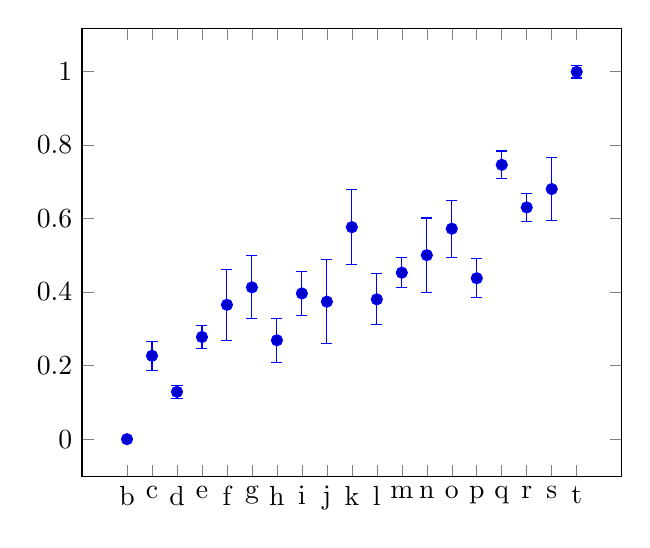
\begin{tikzpicture}
\begin{axis}[%
	%grid=both,%
	%xmajorgrids,%
	xtick={1,2,3,4,5,6,7,8,9,10,11,12,13,14,15,16,17,18,19},%
	xticklabels={b,c,d,e,f,g,h,i,j,k,l,m,n,o,p,q,r,s,t},%
]
% Line plot
\addplot
	plot[ 	%smooth,
	   		only marks,
	      	error bars/.cd,
	      	y dir=both, y explicit %
		]
	coordinates{
	(1,0) 			+- (0,0)
	(2,0.226697)	+- (0,0.0389)
	(3,0.128649)	+- (0,0.0174)
	(4,0.277819)	+- (0,0.0316)
	(5,0.365309) 	+- (0,0.0960)
	(6,0.412726)	+- (0,0.0856)
	(7,0.268849) 	+- (0,0.0598)
	(8,0.396237)	+- (0,0.0589)
	(9,0.373823)	+- (0,0.1148)
	(10,0.576375)	+- (0,0.1020)
	(11,0.380172) 	+- (0,0.0696)
	(12,0.452672)	+- (0,0.0404)
	(13,0.500303)	+- (0,0.1010)
	(14,0.572158)	+- (0,0.0778)
	(15,0.437586)	+- (0,0.0524)
	(16,0.745885)	+- (0,0.0376)
	(17,0.630023)	+- (0,0.0386)
	(18,0.679989)	+- (0,0.0852)
	(19,0.998734)	+- (0,0.0169)
};

\end{axis}
\end{tikzpicture}


% plot erstellt mit MATLAB-File p:\doc\MATLAB\WFS-CompareDMPs\wfs_Compare2008c.m (FromToTo = 1:5:1024)
% und matlab2tikz

%[ 1:19;std(NormCumulativeError);mean(NormCumulativeError)]
%
%ans =
%
%  Columns 1 through 12
%
%    1.0000    2.0000    3.0000    4.0000    5.0000    6.0000    7.0000    8.0000    9.0000   10.0000   11.0000   12.0000
%         0    0.0389    0.0174    0.0316    0.0960    0.0856    0.0598    0.0589    0.1148    0.1020    0.0696    0.0404
%         0    0.2267    0.1286    0.2778    0.3653    0.4127    0.2688    0.3962    0.3738    0.5764    0.3802    0.4527
%
%  Columns 13 through 19
%
%   13.0000   14.0000   15.0000   16.0000   17.0000   18.0000   19.0000
%    0.1010    0.0778    0.0524    0.0376    0.0386    0.0852    0.0169
%    0.5003    0.5722    0.4376    0.7459    0.6300    0.6800    0.9987          	
         	
%
%\end{preview}
%\end{document}%
		\label{fig:NormalizedErrorPlot}%
	\end{figure}%
\else
	\begin{figure}[htp]
		\centering
		%\documentclass{article}
%\usepackage{tikz,pgfplots}
%\usepackage[pdftex,active,tightpage]{preview}
%\begin{document}
%\begin{preview}

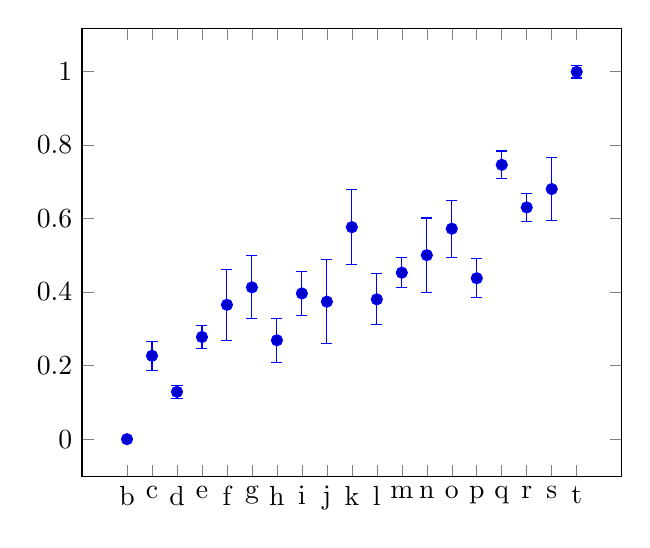
\begin{tikzpicture}
\begin{axis}[%
	%grid=both,%
	%xmajorgrids,%
	xtick={1,2,3,4,5,6,7,8,9,10,11,12,13,14,15,16,17,18,19},%
	xticklabels={b,c,d,e,f,g,h,i,j,k,l,m,n,o,p,q,r,s,t},%
]
% Line plot
\addplot
	plot[ 	%smooth,
	   		only marks,
	      	error bars/.cd,
	      	y dir=both, y explicit %
		]
	coordinates{
	(1,0) 			+- (0,0)
	(2,0.226697)	+- (0,0.0389)
	(3,0.128649)	+- (0,0.0174)
	(4,0.277819)	+- (0,0.0316)
	(5,0.365309) 	+- (0,0.0960)
	(6,0.412726)	+- (0,0.0856)
	(7,0.268849) 	+- (0,0.0598)
	(8,0.396237)	+- (0,0.0589)
	(9,0.373823)	+- (0,0.1148)
	(10,0.576375)	+- (0,0.1020)
	(11,0.380172) 	+- (0,0.0696)
	(12,0.452672)	+- (0,0.0404)
	(13,0.500303)	+- (0,0.1010)
	(14,0.572158)	+- (0,0.0778)
	(15,0.437586)	+- (0,0.0524)
	(16,0.745885)	+- (0,0.0376)
	(17,0.630023)	+- (0,0.0386)
	(18,0.679989)	+- (0,0.0852)
	(19,0.998734)	+- (0,0.0169)
};

\end{axis}
\end{tikzpicture}


% plot erstellt mit MATLAB-File p:\doc\MATLAB\WFS-CompareDMPs\wfs_Compare2008c.m (FromToTo = 1:5:1024)
% und matlab2tikz

%[ 1:19;std(NormCumulativeError);mean(NormCumulativeError)]
%
%ans =
%
%  Columns 1 through 12
%
%    1.0000    2.0000    3.0000    4.0000    5.0000    6.0000    7.0000    8.0000    9.0000   10.0000   11.0000   12.0000
%         0    0.0389    0.0174    0.0316    0.0960    0.0856    0.0598    0.0589    0.1148    0.1020    0.0696    0.0404
%         0    0.2267    0.1286    0.2778    0.3653    0.4127    0.2688    0.3962    0.3738    0.5764    0.3802    0.4527
%
%  Columns 13 through 19
%
%   13.0000   14.0000   15.0000   16.0000   17.0000   18.0000   19.0000
%    0.1010    0.0778    0.0524    0.0376    0.0386    0.0852    0.0169
%    0.5003    0.5722    0.4376    0.7459    0.6300    0.6800    0.9987          	
         	
%
%\end{preview}
%\end{document}
	\caption{%
		Plot of normalized difference Value ($E_{i_{norm}}$, blue diamonds) for the 19 scanned protocols overlaid over Quality-plot (red dots) obtained from the simulation. The normalized Error has been calculated using the difference image of each protocol $i$ with protocol B. The error bars for each protocol show the standard deviation of the error calculated for 205 of the 1024 slices. Note that the scale of the error been normalized to 20--\SI{100}{\percent}, so that both the quality from the simulation and the error are directly comparable. The abscissa shows the scanning time in percentage of time used for the gold standard scan. Protocol T corresponds to the fastest scanning time, protocol B to the slowest. The protocols inbetween are shown in decreasing order from T--B for increasing percentage of the scanning time.%
		}%
		\label{fig:NormalizedErrorPlot}
	\end{figure}
\fi

\subsubsection{Three dimensional visualization of different protocols}%
\label{subsec:comparison}%
The tomograms of the different protocols have been three dimensionally analyzed and visualized using MeVisLab (Version 2.0 (2009-06-09 Release), MeVis Medical Solutions AG and Fraunhofer MEVIS � Institute for Medical Image Computing, Bremen, Germany). Airway segments have been extracted using a threshold interval based region growing algorithm. A seed point for the region growing algorithm has been manually defined in the most proximal slice for each independent airway segment. The coordinates of the seed points have been kept constant for protocol B--T, allowing direct comparison of the airway segment reconstructions of the different protocols. Airway segments extracted for protocol B, L and T are shown in figure~\ref{fig:BvsT}.

The data shown in figure~\ref{fig:BvsT} represent three of the 19 scanned protocols. Protocol B corresponds to a slightly oversampled gold standard scan, obtained with 15732 projections for all three subscans, recorded in \SI{66}{\minute}. Protocol L has been obtained in \SI{35}{\minute} with total 7866 projections. Protocol T has been obtained in \SI{12}{\minute} with total 2185 projections. The tomographic dataset from protocol B has been reconstructed from 5244 merged projection images, the dataset from protocol L has been reconstructed from 2622 merged projections and the dataset from protocol T has been reconstructed using only 874 merged projections. Even if we scanned protocols L and T while violating the sampling theorem and with a total scanning time reduction of \SI{40}{\percent} or more than \SI{86}{\percent}, the samples still appear to be identical to the gold standard protocol in the low-resolution three dimensional visualization as shown in figure~\ref{fig:BvsT}(a), (b) and (c).

Obviously, the artifacts introduced through the reduction in scanning time only become apparent at higher magnification. The blue cube inside the green airway segments in figures~\ref{fig:BvsT}(a), (b) and (c) are shown as isosurface visualizations of the lung tissue (which exactly corresponds to the negative of the extracted airway segment) in figures~\ref{fig:BvsT}(d), (e) and (f). The regions of interest show a cube with a side length of \SI{379}{\micro\meter} or 256 pixels.

Even with the higher magnification, the reconstructions of protocol L in figure~\ref{fig:BvsT}(e) appears nearly identical to the reconstruction of the region of interest of protocol B (fig.~\ref{fig:BvsT}(d)). We observe that the isosurface of the region of interest of protocol T shown in figure~\ref{fig:BvsT}(f) appears rougher than the isosurface of protocol B. This roughness is introduced through wave-like artifacts visible in the original slice of the dataset of protocol T (not shown) which arise through the breaching of the sampling theorem, since we have only acquired 874 projections for the two ring-scans instead of the 5139 projections ($(3072-200)\frac{\pi}{2}$) which would be necessary to satisfy the sampling theorem. But even with this strong undersampling a segmentation, three dimensional reconstruction and visualization of the sample is still possible. Thus, if the user desires to gain a quick overview over his sample at a high resolution, e.g.\ to quickly assess the integrity of multiple samples over a short time, such a time-saving protocol could be used. It has to be mentioned, that a quick overview could, in principle, also be obtained with a low-resolution scan, which usually automatically accommodates a larger field of view. However, the resolution would not be sufficient to detect interesting features.

\onecolumn%
\ifiucr%%% iucr %%%
	\begin{figure}%
		\centering%
		\caption{%
			Comparison of three-dimensional visualizations of protocols B, L and T. %
		(a) Three independent airway segments (green, red, yellow) of Protocol B have been extracted using a region growing algorithm. %
		(b) Same for protocol L. %
		(c) Same for protocol T. A cubical region of interest (ROI, blue) with a side length of 256 pixels (corresponding to \SI{379}{\micro\meter}) is marked inside the leftmost segment for all protocols. %
		(d): Detailed view of isosurfaces of the lung tissue inside the ROIs shown for protocol B. %
		(e): Same for protocol L.
		(f): Same for protocol T. Note the artifacts in the isosurface in subfigure (e) and (f).%
		}%
		\renewcommand{\imsize}{.333\linewidth}%
		\pgfmathsetlength{\imagewidth}{\imsize}%
		\pgfmathsetlength{\imagescale}{\imagewidth/1085}%
		\def\x{651} % scalebar-x at golden ratio of x=1085px (-20px to fit to width...)
		\def\y{530} % scalebar-y at 90% of height of y=589px
		\begin{tikzpicture}[x=\imagescale,y=-\imagescale]
			\node[anchor=north west,inner sep=0pt,outer sep=0pt] at (0,0)
				{\includegraphics[width=\imagewidth]{img/comparisonBvsT/ob}};
			% 1030px = 2.627mm > 100px = 255um > 196px = 500um
%			\draw[|-|,thick] (30,339) -- (1054,454) node [white,sloped,midway,above] {\SI{2.627}{\milli\meter} (1775px)};
			\draw [|-|,thick] (\x,\y) -- (\x+196,\y) node [fill=white,semitransparent,right] {\SI{500}{\micro\meter}};
			\draw [|-|,thick] (\x,\y) -- (\x+196,\y) node [right] {\SI{500}{\micro\meter}};
			\node [anchor=south west] at (0,589) {(a)};
		\end{tikzpicture}%
		\begin{tikzpicture}[x=\imagescale,y=-\imagescale]%
			\node[anchor=north west,inner sep=0pt,outer sep=0pt] at (0,0)
				{\includegraphics[width=\imagewidth]{img/comparisonBvsT/ol}};
			% 1030px = 2.627mm > 100px = 255um > 196px = 500um
			\draw [|-|,thick] (\x,\y) -- (\x+196,\y) node [fill=white,semitransparent,right] {\SI{500}{\micro\meter}};
			\draw [|-|,thick] (\x,\y) -- (\x+196,\y) node [right] {\SI{500}{\micro\meter}};
			\node [anchor=south west] at (0,589) {(b)};
		\end{tikzpicture}%
		\begin{tikzpicture}[x=\imagescale,y=-\imagescale]%
			\node[anchor=north west,inner sep=0pt,outer sep=0pt] at (0,0)
				{\includegraphics[width=\imagewidth]{img/comparisonBvsT/ot}};
			% 1030px = 2.627mm > 100px = 255um > 196px = 500um
			\draw [|-|,thick] (\x,\y) -- (\x+196,\y) node [fill=white,semitransparent,right] {\SI{500}{\micro\meter}};
			\draw [|-|,thick] (\x,\y) -- (\x+196,\y) node [right] {\SI{500}{\micro\meter}};
			\node [anchor=south west] at (0,589) {(c)};
		\end{tikzpicture}%
		\\%
		\renewcommand{\imsize}{.333\linewidth}%
		\pgfmathsetlength{\imagewidth}{\imsize}%
		\pgfmathsetlength{\imagescale}{\imagewidth/816}%
		\def\x{504} % scalebar-x at golden ratio of x=816px
		\def\y{734} % scalebar-y at 90% of height of y=815px
		\begin{tikzpicture}[x=\imagescale,y=-\imagescale]%
			\node[anchor=north west,inner sep=0pt,outer sep=0pt] at (0,0)
				{\includegraphics[width=\imagewidth]{img/comparisonBvsT/roiB}};
			% 761px = 0.37888mm > 100px = 50um > 100.4px = 500um
%			\draw[|-|,thick] (792,438) -- (31,435) node [sloped,midway,above] {\SI{378.88}{\micro\meter} (256px)};
			\draw[|-|,thick] (\x,\y) -- (\x+100.4,\y) node [fill=white,semitransparent,right] {\SI{50}{\micro\meter}};
			\draw[|-|,thick] (\x,\y) -- (\x+100.4,\y) node [right] {\SI{50}{\micro\meter}};
			\node [fill=white,semitransparent,anchor=south west] at (0,815) {(d)};
			\node [anchor=south west] at (0,815) {(d)};
		\end{tikzpicture}%
		\begin{tikzpicture}[x=\imagescale,y=-\imagescale]%
			\node[anchor=north west,inner sep=0pt,outer sep=0pt] at (0,0)
				{\includegraphics[width=\imagewidth]{img/comparisonBvsT/roiL}};
			% 761px = 0.37888mm > 100px = 50um > 100.4px = 500um
			\draw[|-|,thick] (\x,\y) -- (\x+100.4,\y) node [fill=white,semitransparent,right] {\SI{50}{\micro\meter}};
			\draw[|-|,thick] (\x,\y) -- (\x+100.4,\y) node [right] {\SI{50}{\micro\meter}};
			\node [fill=white,semitransparent,anchor=south west] at (0,815) {(e)};
			\node [anchor=south west] at (0,815) {(e)};
		\end{tikzpicture}%
		\begin{tikzpicture}[x=\imagescale,y=-\imagescale]%
			\node[anchor=north west,inner sep=0pt,outer sep=0pt] at (0,0)
				{\includegraphics[width=\imagewidth]{img/comparisonBvsT/roiT}};
			% 761px = 0.37888mm > 100px = 50um > 100.4px = 500um
			\draw[|-|,thick] (\x,\y) -- (\x+100.4,\y) node [fill=white,semitransparent,right] {\SI{50}{\micro\meter}};
			\draw[|-|,thick] (\x,\y) -- (\x+100.4,\y) node [right] {\SI{50}{\micro\meter}};
			\node [fill=white,semitransparent,anchor=south west] at (0,815) {(f)};
			\node [anchor=south west] at (0,815) {(f)};
		\end{tikzpicture}%
		\label{fig:BvsT}%
	\end{figure}%
\else%
	\begin{figure}[htp]
		\centering
		\renewcommand{\imsize}{.333\linewidth}%
		\includegraphics[width=\imagewidth]{img/comparisonBvsT/ob}%
		\includegraphics[width=\imagewidth]{img/comparisonBvsT/ol}%
		\includegraphics[width=\imagewidth]{img/comparisonBvsT/ot}%
		\\%
		\includegraphics[width=\imagewidth]{img/comparisonBvsT/roiB}%
		\includegraphics[width=\imagewidth]{img/comparisonBvsT/roiL}%
		\includegraphics[width=\imagewidth]{img/comparisonBvsT/roiT}%
		\caption{%
			Comparison of three-dimensional visualizations of protocols B, L and T. %
		(a) Three independent airway segments (green, red, yellow) of Protocol B have been extracted using a region growing algorithm. %
		(b) Same for protocol L. %
		(c) Same for protocol T. A cubical region of interest (ROI, blue) with a side length of 256 pixels (corresponding to \SI{379}{\micro\meter}) is marked inside the leftmost segment for all protocols. %
		(d): Detailed view of isosurfaces of the lung tissue inside the ROIs shown for protocol B. %
		(e): Same for protocol L.
		(f): Same for protocol T. Note the artifacts in the isosurface in subfigure (e) and (f).%
		}%
		\label{fig:BvsT}%
	\end{figure}
\fi%
\twocolumn%

The field of view can be increased even further; we also scanned and reconstructed a rat lung sample with 5 scanning positions, resulting in a five-fold (4.74$\times$) increase in available field of view from 1024$\times$1024 pixels to 4852$\times$4852 pixels (data not shown). We have been able to reconstruct a sample with size of approximately 0.82$\times$7.18$\times$\SI{1.52}{\milli\meter} (cropped to 552$\times$4852$\times$1024 pixels) at a voxel side length of \SI{1.48}{\micro\meter}.